%%%%%%%%%%%%%%%%%%%%%%%%%%%%%%%%%%%%%%%%%%%%%%%%%%%%%%%%%%%%%%%%%%%%%
\begin{frame}{Motivating Scenarios}
    .\hspace{0.2cm}Schooling in fish
    %\footnote{https://rememberfukushima.org/fallout-maps/}
    \hspace{2.1 cm}
    Deep Water Horizon (2010)
    %\footnote{https://response.restoration.noaa.gov}
    \\
	\begin{minipage}{0.45\textwidth}	
		\begin{figure}
			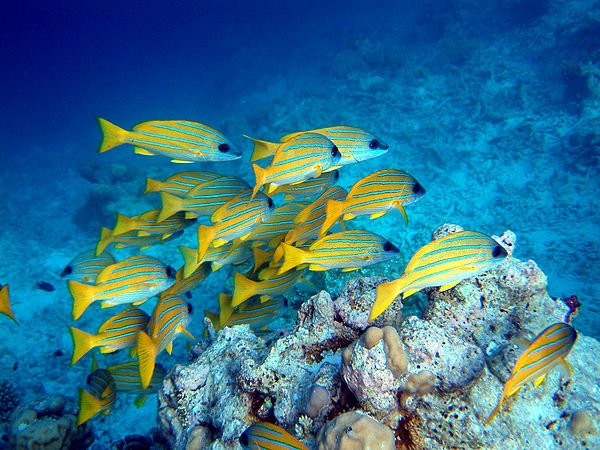
\includegraphics[width=0.9\textwidth]{figures/schooling_fish.jpg}
			%\caption{Oil Spills}
			%\label{fig:schools_of_fish}
		\end{figure}
		\begin{figure}
			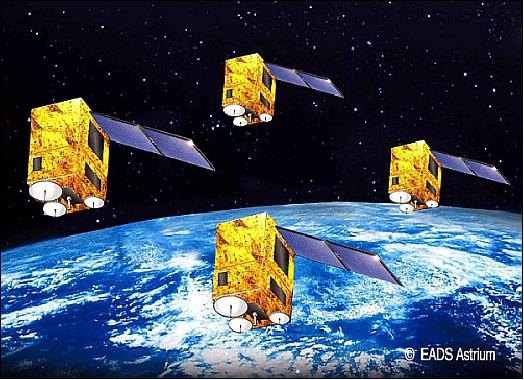
\includegraphics[scale=0.2]{figures/Essaim_constellation.jpg}\label{fig:satellite_flock}
		\end{figure}
	\end{minipage}
	\hspace{0.05cm}
	\begin{minipage}{0.45\textwidth}
		\begin{figure}
			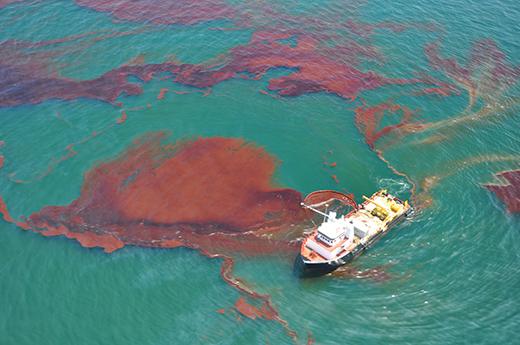
\includegraphics[width=\textwidth]{figures/oil_spill.jpg}
			%\caption{Oil Spills}
			%\label{fig:oilspills}
		\end{figure}
		\begin{figure}
			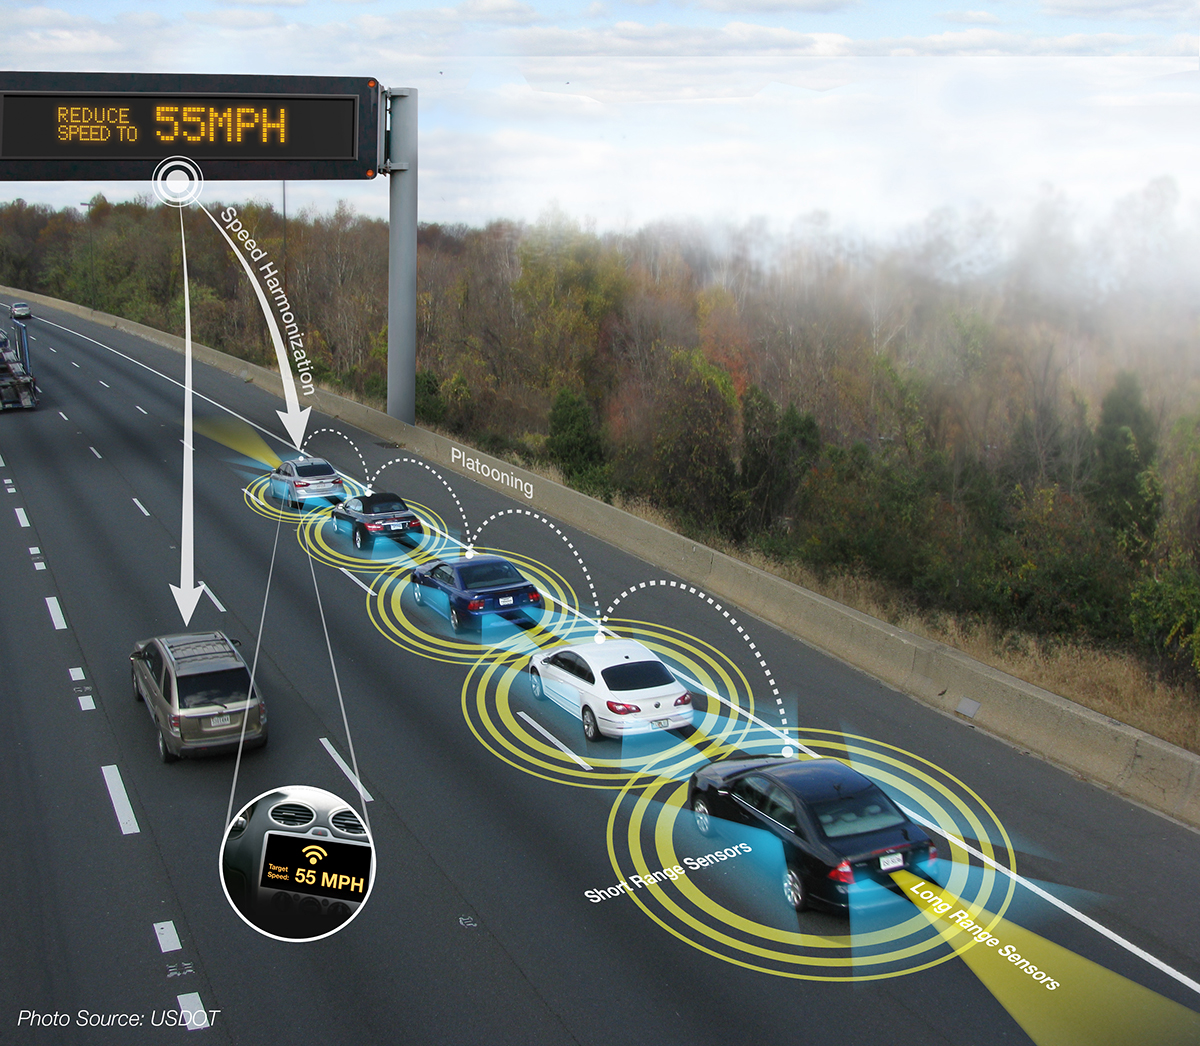
\includegraphics[scale=0.20]{figures/Platooning.jpg}	
			\label{fig:Platooning}
		\end{figure}	
	\end{minipage} 

 .
 \hspace{0.2 cm}
  EADS Astrium 
 %\footnote{https://earth.esa.int}
\hspace{2.7 cm}
Vehicle Platoons
\\
\end{frame}
%%%%%%%%%%%%%%%%%%%%%%%%%%%%%%%%%%%%%%%%%%%%%%%%%%%%%%%%%%%%%%%%%%%%%
%%%%%%%%%%%%%%%%%%%%%%%%%%%%%%%%%%%%%%%%%%%%%%%%%%%%%%%%%%%%%%%%%%%%%
\begin{frame}{Physical Agent Dynamics}	
	\begin{minipage}{0.3\textwidth}	
		\begin{figure}
			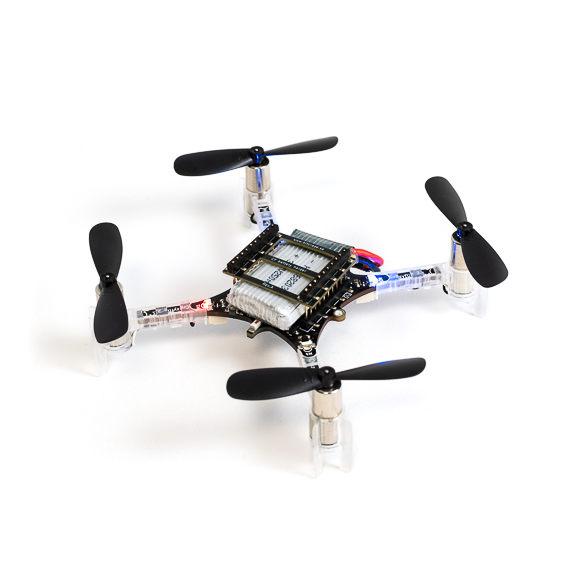
\includegraphics[width=0.9\textwidth]{figures/crazyflie_2_1_585px.jpg}
			\caption{Crazyflie}
			%\label{fig:schools_of_fish}
		\end{figure}
	\end{minipage}
	\hspace{0.05cm}
	\begin{minipage}{0.3\textwidth}
		\begin{figure}
			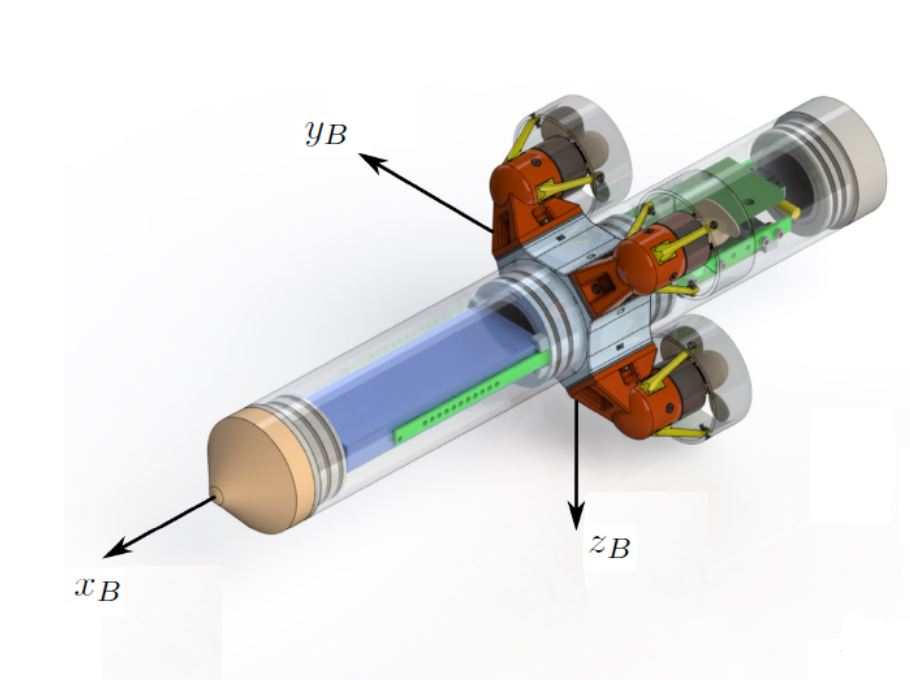
\includegraphics[width=\textwidth]{figures/Hippocampus.jpg}
			\caption{Hippocampus}
			%\label{fig:oilspills}
		\end{figure}	
	\end{minipage}
	\hspace{0.05cm}
	\begin{minipage}{0.3\textwidth}
		\begin{figure}
			\includegraphics[width=\textwidth]{figures/zooids.jpg}
			\caption{Zooids}
			%\label{fig:oilspills}
		\end{figure}	
	\end{minipage}
	\begin{itemize}		
		\item Single/double integrator dynamics
		\item Linear Time Invariant (LTI)/Linear Parameter Varying (LPV) dynamics
		\item with/ without non-holonomic constraints
	\end{itemize}
\end{frame}
%%%%%%%%%%%%%%%%%%%%%%%%%%%%%%%%%%%%%%%%%%%%%%%%%%%%%%%%%%%%%%%%%%%%%
%%%%%%%%%%%%%%%%%%%%%%%%%%%%%%%%%%%%%%%%%%%%%%%%%%%%%%%%%%%%%%%%%%%%%
\begin{frame}{Core Idea}	
	\begin{itemize}
		\item Control of a single non-linear (possibly non-holonomic) agent: Well-studied problem and various techniques are known
		\begin{itemize}
			\item LPV
			\item Dynamic-inversion
			\item Flatness-based control
		\end{itemize}		
		\item About 3 decades of work on studying interconnections of "simple" agent dynamics where simple could mean
		\begin{itemize}
			\item single/ double integrator dynamics
			\item positive systems 
		\end{itemize} 
	\end{itemize}
\pause
\textbf{Key questions:}
\begin{itemize}
	\item Can we maintain this separation in the controller design? i.e design local agent controllers and study the interconnections of these closed loop "simplified" systems
	\item Can we give some stability and performance guarantees with such a strategy?
	\item What kind of control architectures are possible?
	\end{itemize}
\end{frame}
%%%%%%%%%%%%%%%%%%%%%%%%%%%%%%%%%%%%%%%%%%%%%%%%%%%%%%%%%%%%%%%%%%%%%
%%%%%%%%%%%%%%%%%%%%%%%%%%%%%%%%%%%%%%%%%%%%%%%%%%%%%%%%%%%%%%%%%%%%%
\begin{frame}{Different Control Architectures}	
	\begin{minipage}{0.46\textwidth}	
		\begin{figure}
			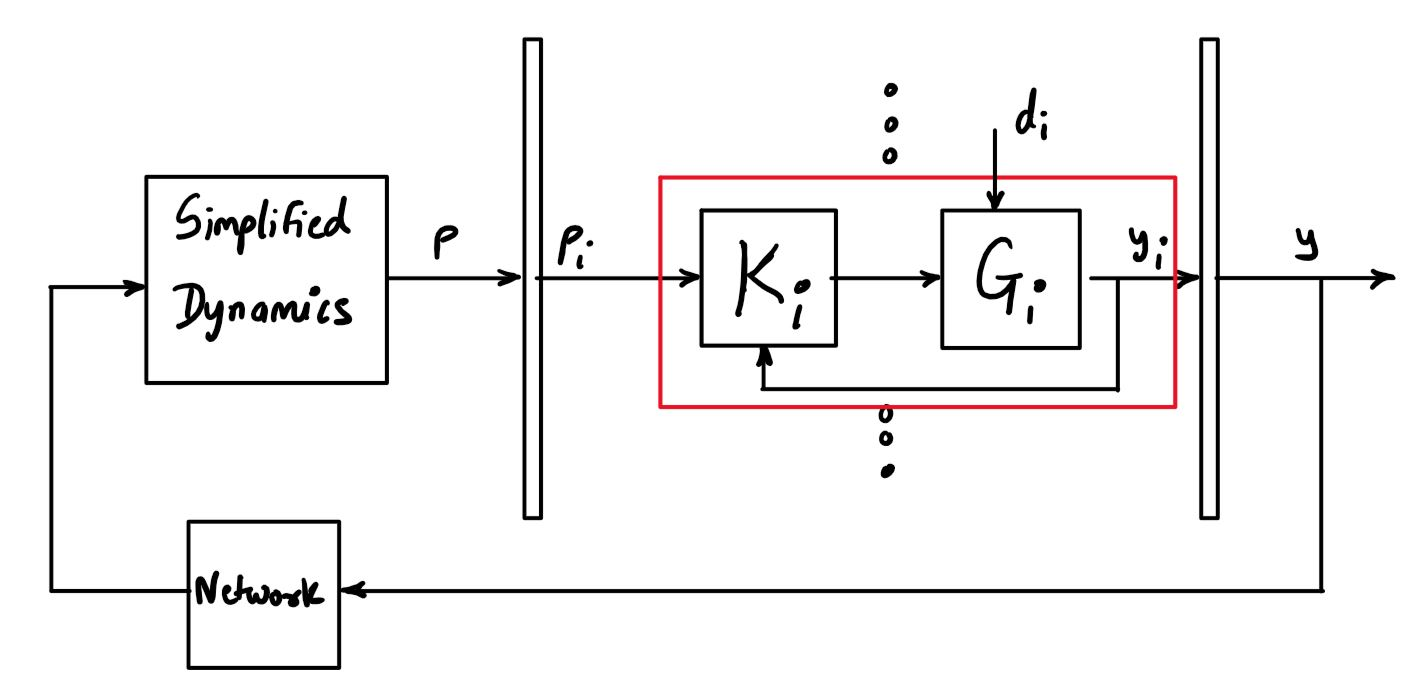
\includegraphics[scale=0.30]{figures/Coupled.jpg}	
			\label{fig:Coupled}
		\end{figure}	
		Coupled architecture
		\begin{itemize}
		\item Relative distances important
		\item Small inter-agent distances
		\item High disturbances
		\end{itemize}
	\end{minipage}
	\hspace{0.5cm}
	\begin{minipage}{0.46\textwidth}
		\begin{figure}
			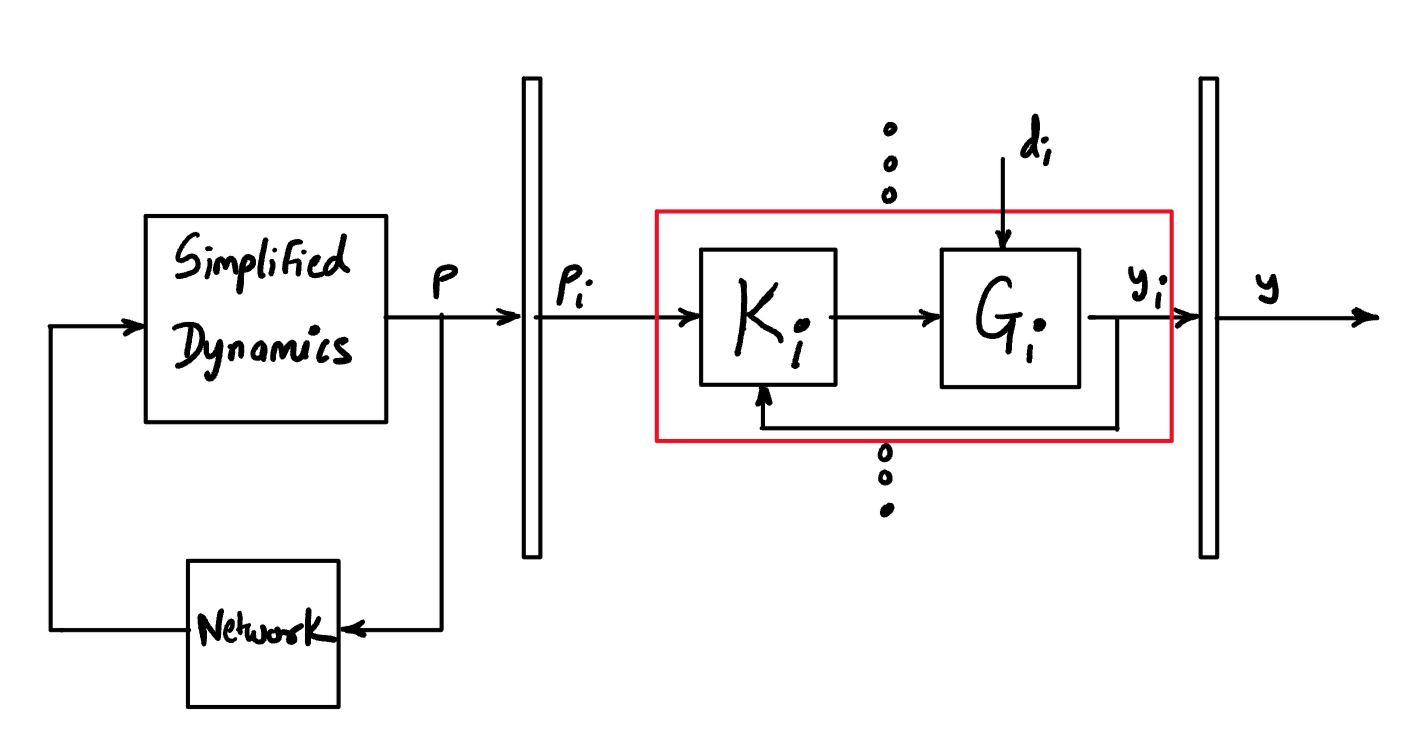
\includegraphics[scale=0.30]{figures/Decoupled.jpg}	
			\label{fig:Decoupled}
		\end{figure}	
		Decoupled architecture
		\begin{itemize}
			\item Absolute COM position important 
			\item Large inter-agent distances
			\item Low disturbances
		\end{itemize}
	\end{minipage}  
\end{frame}